\documentclass{article}

\usepackage[preprint]{neurips_2023}
\usepackage{caption} % to use \captionsetup
\DeclareCaptionFormat{myformat}{\textbf{#1 #2} #3}
% \DeclareCaptionJustification{outside}{\hspace{-3cm}} 
\captionsetup{format=myformat}
% \captionsetup{justification   = raggedright, % shift caption to the left
%               singlelinecheck = false}
\usepackage{shortcuts}


\title{Semantic Classification of 3D point clouds with multiscale spherical neighborhoods \\ \vspace{.3cm}
\small{NPM3D project report}
}

\author{%
  Inès ~Vati\thanks{Engineering student from École des Ponts ParisTech, Champs-sur-Marne, France} \\
  MVA, ENS Paris-Saclay, Cachan, France\\
  \texttt{\email{ines.vati@eleves.enpc.fr}}
}

\date{}

\begin{document}
\maketitle

\begin{abstract}
    The project consists in studying the article from Thomas et al. \cite{thomas_semantic_2018} by implementing it and proposing improvements. The goal of the studied article is to classify each point of a 3D point clouds using an innovative approach to design features which will be used to train a random forest classifier. 
    [what i did]
    As no code were provided, the methods were implemented from scratch. The code implemented for this project is available on \url{https://github.com/InesVATI/npm3d-project}. 
\end{abstract}
\textbf{Keywords.} 3D point clouds, semantic classification, multiscale, spherical neighborhoods, Random Forest Classifier


% \section{Introduction}

\section{Proposed method}

In their study \cite{thomas_semantic_2018}, the authors employ a multiscale approach to design informative features, drawing upon the findings of Hackel et al. in 2016 \cite{hackel_fast_nodate}, which demonstrated the improved efficiency of such an approach over adapting the scale for each point \cite{weinmann_semantic_2015}. To compute these features, the authors adopt a spherical definition of neighborhoods, incorporating neighbors within a radius that exponentially increases with the scale $s$, denoted as $r_s = r_0 * \phi^s$. This formulation ensures that the neighborhoods appropriately reflect the density of the point cloud. 

Let's consider a set of $N$ points of interest for which we aim to compute the multiscale features. For each scale, the same set of $N_{feats}$ features is computed, as detailed in Table \ref{tab:thomas_feat}. $S$ is the number of scales. The feature computation proceeds through the following steps:

\begin{enumerate}
    \item At scale 0, the eigenvalues and eigenvectors of the covariance matrix of the neighborhood, obtained with an initial radius $r_0$, are computed. Subsequently, the features for each point of interest are derived using the formulas outlined in Table \ref{tab:thomas_feat}.
    \item  For each scale $s$, a grid subsampling is applied to the original cloud using a voxel size of $r/\rho$. Each original point is then assigned to the closest voxel center, inheriting the features of the voxel center for that particular scale. 
    \item The $N_{feats}$ features are computed for each voxel center associated with at least one point of interest from the original point cloud, within a spherical neighborhood of radius $r_s = r_0 * \phi^s$.
    \item Consequently, we obtain a feature matrix of size $N \times N_{feats} * S$.
\end{enumerate}
Here, $\phi$ is the ratio between the radius of consecutive neighborhoods and $\rho$ is the ratio between the radius of the spherical neighborhood and the voxel size of the grid subsampling. $\rho$ enables to control the maximum number of subsampled points that a neighborhood can contain.

\begin{table}[H]
    \centering
    \begin{tabular}{|c||c|}
    \hline
    \textbf{Feature} & \textbf{Formula} \\
    \hline   
    Sum of eigenvalues & $\sum \lambda_i$ \\[1ex]
    % \hline
    Omnivariance & $(\prod \lambda_i)^{(1/3)}$\\[1ex]
    % \hline
    Eigenentropy & $-\sum \lambda_i \ln(\lambda_i)$\\[1ex]
    % \hline
    Linearity & $\frac{\lambda_1 - \lambda_2}{\lambda_1}$\\[1ex]
    % \hline
    Planarity & $\frac{\lambda_2 - \lambda_3}{\lambda_1}$\\[1ex]
    % \hline
    Sphericity & $\frac{\lambda_3}{\lambda_1}$\\[1ex]
    % \hline
    Change of curvature & $\lambda_1 - \lambda_3$\\[1ex]
    % \hline
    Verticality ($\times2$) & $|\arcsin(\dotp{e_i}{e_z})|_{i=1, 3}$ \\[1ex]
    % \hline
    Absolute moment ($\times6$) & $\frac{1}{|\mathcal{N}|}|\sum_{j\in\mathcal{N}} \dotp{p_j - \mathbf{p}}{e_i}^k|_{k = 1, 2;\; i = 1, 2, 3}$\\[1ex]
    % \hline  
    Vertical moment ($\times2$) & $\frac{1}{|\mathcal{N}|}|\sum_{j\in\mathcal{N}} \dotp{p_j - \mathbf{p}}{e_z}^k|_{k=1, 2}$ \\[1ex]
    % \hline
    Number of points & $|\mathcal{N}|$\\[1ex]
    \hline
    \end{tabular}
    \caption{$N_{feats}=18$ Geometric features \cite{thomas_semantic_2018} of point $\mathbf{p}$. $\lambda_i$ are the eigenvalues of the covariance matrix of the neighborhood $\mathcal{N}$ of $\mathbf{p}$, sorted in decreasing order. $e_i$ are the corresponding eigenvectors.}
    \label{tab:thomas_feat}
\end{table}

\begin{table}[H]
    \centering
    \begin{tabular}{|c||c|}
        \hline
    \textbf{Feature} & \textbf{Formula} \\
        \hline
        Vertical range & $z_{max} - z_{min} $\\[1ex]
        % \hline
        Height below & $\mathbf{p}_z - z_{min} $ \\[1ex]
        % \hline
        Height above & $z_{max} - \mathbf{p}_z$\\[1ex]
        \hline
    \end{tabular}

    \caption{Additional height features from \cite{hackel_fast_nodate, mohamed_improvement_2022}, where $z_{max} = \umax{j\in\mathcal{N}}p_{j,z}$ and $z_{min} = \umin{j\in\mathcal{N}} p_{j,z}$. $\N$ is the neighborhood of point $\mathbf{p}$. $p_{j,z}$ is the coordinate of point $j$ in the vertical axis.}
    \label{tab:height_feat}
\end{table}

\section{Experiments and results}
I used two datasets to evaluate the method: the Paris-rue-Cassette dataset\footnote{\url{http://data.ign.fr/benchmarks/UrbanAnalysis/}}, a point cloud of 12 million points and the NPM3D dataset\footnote{\url{https://npm3d.fr/benchmark-for-master-course-on-3d-point-clouds}}, that groups three point clouds, including the MiniLille and MiniParis point clouds. The MiniLille dataset has 1,901,853 and 2,500,428 points and the MiniParis dataset has 4,159,318 points. 

The Paris-rue-Cassette dataset serves as the basis for comparing various methods.After carefully selecting parameters for a Random Forest classifier, I applied the same classifier configuration to investigate the following:
\begin{itemize}
    \item The predictive performance, comparing the use of a spherical neighborhood versus a K-Nearest Neighbors (KNN) neighborhood (detailed in Section \ref{sec:compare_neigh_def}).
    \item The impact of using multiple scales, comparing the proposed method with and without multiscaling (outlined in Section \ref{sec:w/o_multiscale}).
    \item The significance of features and the potential benefits of incorporating additional height features, as suggested by Mohamed et al. \cite{mohamed_improvement_2022} (explored in Section \ref{sec:compare_w/o_height}).
\end{itemize}
For all the experiments, the tree classifier employed 150 trees and the Gini criterion. In addition, balanced class weights were used to address class imbalances, with weights being inversely proportional to class frequencies in the input data. Notably, no maximum depth constraint were set, as this led to better results across all approaches. Consequently, nodes were expanded until either all leaves were pure or until each leaf contained fewer than two samples.
    
Furthermore, the NPM3D dataset is used in Section \ref{sec:generalization} to assess the method's generalization ability to datasets not involved in classifier training.

To assess the performance of the different approaches, the Intersection over Union (IoU) metric or jaccard index is used. It is given by 
$$
\textrm{IoU} = \frac{\textrm{TP}}{\textrm{TP} + \textrm{FP} + \textrm{FN}}
$$
where $TP$ is the number of true positive, $FP$ the number of false positive and $FN$ the number of false negative. I also computed the weighted IoU which is the mean of the IoU for each class, weighted by the number of points of each class. As performed in \cite{thomas_semantic_2018}, the experiments were repeated 10 times and the mean and standard deviation of the Intersection over Union (IoU) metric were computed and are presented in Tables \ref{tab:benchmark_RF} and \ref{tab:benchmark_Boosting}.

\subsection{Paris-rue-cassette dataset}
The raw ground truth contained a large number of classes. I had to parse an XML file to group together some label classes to fairly compare the results with those obtained in previous studies \cite{thomas_semantic_2018,hackel_fast_nodate,weinmann_semantic_2015}. 

Due to computational constraints, I employed grid subsampling to reduce the size of the point cloud, using a voxel size of 0.1m. The resulting point cloud contains 1,288,215 points. Each voxel center was assigned a label based on the majority label of the points within the voxel. Notably, some classes suffered a significant reduction in the number of points, such as the 'Traffic Sign' label. The number of points per class is given in Table \ref{tab:cassette_label_size}. While it would have been possible to retain all points from these underrepresentated classes in the subsampled point cloud, it is pertinent to explore strategies for managing class imbalances, as discussed in Section \ref{sec:classification}.

\begin{table}[H]
    \begin{center}
            \begin{tabular}{ll}
                    Label & Size \\
                    \hline
                    Ground & 188644 \\
                    Building & 954267 \\
                    Traffic Signs & 195 \\
                    Pedestrians & 2079 \\
                    Cars & 28437 \\
                    Vegetation & 98175 \\
                    Motorcycles & 4523 \\
            \end{tabular}
    \end{center}
    \caption{Class size in Paris-rue-Cassette subsampled cloud}
    \label{tab:cassette_label_size}
\end{table}

On this dataset, I choose $S=4$, $r_0=0.5$m, $\phi=2$, $\rho=5$. The figure \ref{fig:neigh_hist} displays the distribution of the neighborhood sizes in the subsampled cloud at the different scale to check that the neighborhoods are not too small with those parameters. One can notice that some points have very small neighborhoods even without subsampling. However, the neighborhood size is 100 points in average. We can also see that the iterative grid subsampling do not distort too much the neighborhood size distribution. Choosing $S=4$ number of scales seems to be an appropiate choice to avoid having empty neighborhoods while computing the covariance matrix. 

It is worth noting that the radius of the spherical neighborhood adjusts according to the scale, ensuring that the neighborhood consistently represents a fixed portion of space at every scale. This differs from KNN (K-Nearest Neighbors) neighborhood definition, where the neighborhood size is fixed, which can result in an inaccurate description of the neighborhood, particularly at smaller scales.

\begin{figure}
    \begin{subfigure}{0.5\textwidth}
        \centering
        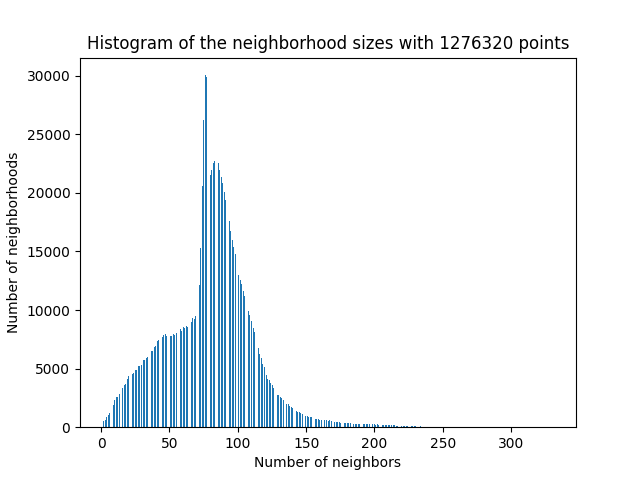
\includegraphics[width=\textwidth]{neigh_hist_scale0.png}
        \caption{$s=0$, $r=0.5m$}
    \end{subfigure}
    \hfill
    \begin{subfigure}{0.5\textwidth}
        \centering
        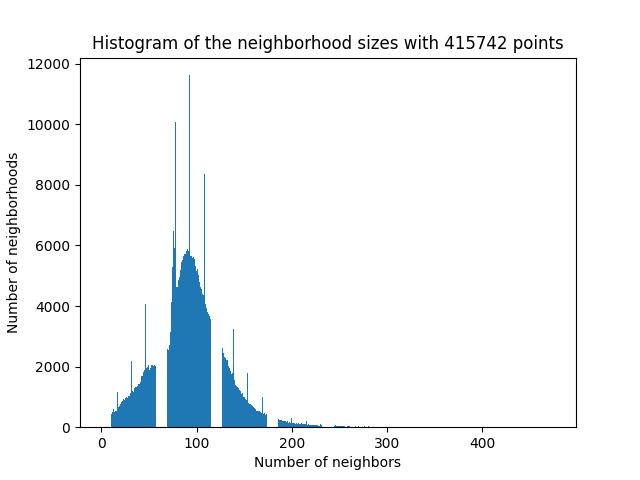
\includegraphics[width=\textwidth]{neigh_hist_scale1.png}
        \caption{$s=1$, $r=1m$}
    \end{subfigure}
    \hfill
    \begin{subfigure}{0.5\textwidth}
        \centering
        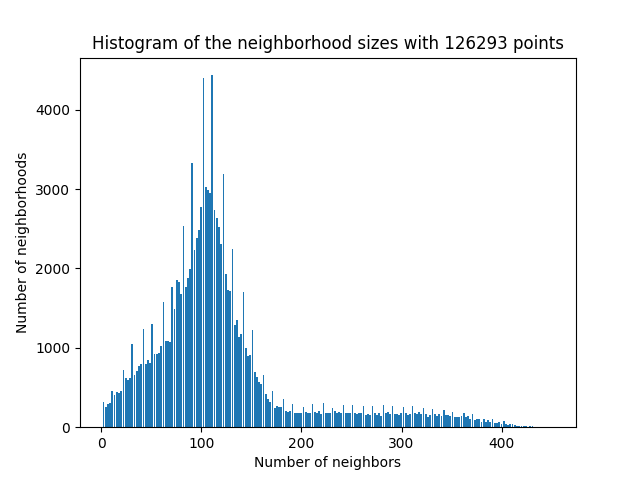
\includegraphics[width=\textwidth]{neigh_hist_scale2.png}
        \caption{$s=2$, $r=2m$}
    \end{subfigure}
    \hfill
    \begin{subfigure}{0.5\textwidth}
        \centering
        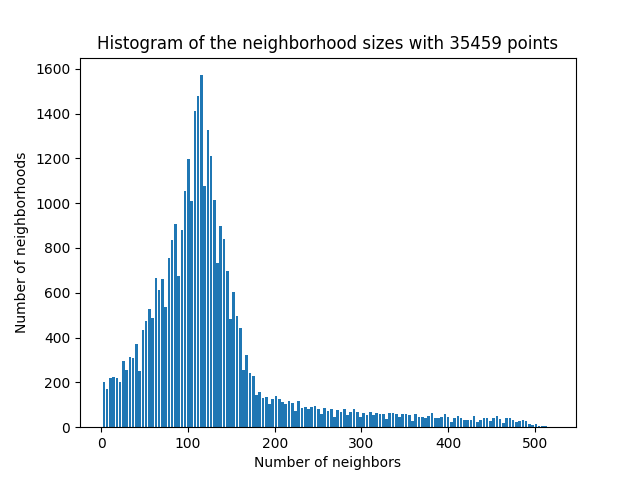
\includegraphics[width=\textwidth]{neigh_hist_scale3.png}
        \caption{$s=3$, $r=4m$}
    \end{subfigure}
    \caption{Histogram of the number of points in the neighborhood of each point for different scales $s$ on the subsampled Paris-rue-Cassette Dataset.}
    \label{fig:neigh_hist}
\end{figure}

\begin{table}
    \hspace*{-3cm}
    \begin{tabular}{cllllllll}
        Method & Ground & Building & Traffic Signs & Pedestrians & Cars & Vegetation & Motorcycles & Weighted IoU \\
        \hline
        \cite{thomas_semantic_2018} & $81.48 \mtiny{\pm 2.95}$ & $71.21 \mtiny{\pm 8.07}$ & $90.25 \mtiny{\pm 11.21}$ & $92.81 \mtiny{\pm 2.00}$ & $47.48 \mtiny{\pm 12.85}$ & $\mathbf{82.34} \mtiny{\pm 4.68}$ & $\mathbf{97.31} \mtiny{\pm 2.27}$ & $78.87 \mtiny{\pm 4.22}$ \\
        + height & $\mathbf{83.16} \mtiny{\pm 2.23}$ & $\mathbf{72.10} \mtiny{\pm 3.60}$ & $\mathbf{97.00} \mtiny{\pm 4.58}$ & $\mathbf{93.56} \mtiny{\pm 1.42}$ & $\mathbf{49.84} \mtiny{\pm 12.70}$ & $81.46 \mtiny{\pm 6.48}$ & $95.23 \mtiny{\pm 2.99}$ & $\mathbf{79.37} \mtiny{\pm 2.95}$ \\
        - multiscale & $68.76 \mtiny{\pm 5.77}$ & $43.25 \mtiny{\pm 3.03}$ & $9.08 \mtiny{\pm 3.18}$ & $71.19 \mtiny{\pm 1.91}$ & $30.12 \mtiny{\pm 4.14}$ & $62.53 \mtiny{\pm 2.57}$ & $54.84 \mtiny{\pm 2.71}$ & $54.74 \mtiny{\pm 1.51}$ \\
        knn & $71.87 \mtiny{\pm 8.28}$ & $57.21 \mtiny{\pm 6.39}$ & $48.24 \mtiny{\pm 27.04}$ & $90.99 \mtiny{\pm 1.98}$ & $36.52 \mtiny{\pm 8.29}$ & $80.76 \mtiny{\pm 1.66}$ & $86.94 \mtiny{\pm 1.52}$ & $70.53 \mtiny{\pm 3.13}$ \\
\end{tabular}
\captionsetup{margin={-3cm, -3cm}}
\caption{ Average IoU (with standard deviation) on the subsampled Paris-rue-Cassette dataset using Random Forest classifier.}
    \label{tab:benchmark_RF}
\end{table}
\begin{table}
    \hspace*{-3cm}
    \begin{tabular}{cllllllll}
        Method & Ground & Building & Traffic Signs & Pedestrians & Cars & Vegetation & Motorcycles & Weighted IoU \\
        \hline
        \cite{thomas_semantic_2018} & $83.34 \mtiny{\pm 2.82}$ & $69.72 \mtiny{\pm 5.91}$ & $58.96 \mtiny{\pm 24.93}$ & $93.37 \mtiny{\pm 2.36}$ & $\mathbf{60.56} \mtiny{\pm 9.58}$ & $77.72 \mtiny{\pm 6.03}$ & $96.04 \mtiny{\pm 2.97}$ & $79.95 \mtiny{\pm 2.73}$ \\
        + height & $\mathbf{84.94} \mtiny{\pm 2.38}$ & $\mathbf{74.30} \mtiny{\pm 6.57}$ & $\mathbf{82.29} \mtiny{\pm 17.82}$ & $\mathbf{94.10} \mtiny{\pm 1.51}$ & $58.91 \mtiny{\pm 12.37}$ & $79.13 \mtiny{\pm 5.79}$ & $\mathbf{97.68} \mtiny{\pm 1.29}$ & $\mathbf{81.52} \mtiny{\pm 3.56}$ \\
        - multiscale & $62.13 \mtiny{\pm 8.48}$ & $41.47 \mtiny{\pm 3.51}$ & $9.06 \mtiny{\pm 1.30}$ & $71.43 \mtiny{\pm 3.35}$ & $28.87 \mtiny{\pm 4.41}$ & $66.50 \mtiny{\pm 1.71}$ & $59.74 \mtiny{\pm 3.04}$ & $54.64 \mtiny{\pm 2.44}$ \\
        knn & $71.06 \mtiny{\pm 9.34}$ & $56.08 \mtiny{\pm 8.58}$ & $37.02 \mtiny{\pm 26.41}$ & $93.68 \mtiny{\pm 2.03}$ & $49.68 \mtiny{\pm 13.76}$ & $\mathbf{81.21} \mtiny{\pm 3.65}$ & $91.35 \mtiny{\pm 3.19}$ & $73.54 \mtiny{\pm 2.73}$ \\
\end{tabular}
\captionsetup{margin={-3cm, -3cm}}
    \caption{Average IoU (with standard deviation) on the subsampled Paris-rue-Cassette dataset using HBG classifier}
    \label{tab:benchmark_Boosting}
\end{table}

\subsection{Comparing Neighborhood Definitions}\label{sec:compare_neigh_def}
By employing spherical neighborhoods instead of KNN, the features represent a consistent portion of space at each scale.

The scores presented in Table \ref{tab:benchmark_RF} shows that the use of spherical neighborhoods consistently outperforms the KNN neighborhood definition. For instance, the 'Traffic Signs' class, the spherical neighborhood approach improved the Jaccard index by nearly 87\% over the KNN neighborhood method. Moreover, the overall weighted IoU is 18\% higher with the spherical neighborhood approach. This highlights the substantial advantage of using spherical neighborhoods in capturing contextual information and enhancing classification accuracy.

Spherical neighborhoods consider points within a 3D spherical region, which inherently captures shape information of the surrounding objects. This additional information can be beneficial for distinguishing between classes with similar appearance but different shapes. Futhermore, the feature given by the number of points in the neighborhood is useless with the KNN neighborhood definition and do not bring any information about the neighborhood occupancy rate. 

\subsection{Impact of Multiscale Features on Performance}\label{sec:w/o_multiscale}
Relying solely on the original scale consistently yields the lowest scores, as demonstrated in Tables \ref{tab:benchmark_RF} and \ref{tab:benchmark_Boosting}. This observation confirms the importance of the multiscale approach. Indeed, using a fixed scale across the scene is inadequate because most scenes contain objects of various sizes. Given the data acquisition process, dense and accurate 3D point clouds exhibiting substantial variations in point density may be expected. This underscores the necessity of considering multiple scales to effectively capture the complexities and variations present in the point cloud.


\subsection{Comparison with Additional Features and Assessment of Feature Importance}\label{sec:compare_w/o_height}

HHeight features, such as vertical range, as listed in Table \ref{tab:height_feat}, were employed in previous studies \cite{hackel_fast_nodate,mohamed_improvement_2022} for their ability to better characterize vertical and thin objects such as traffic signs or tree trunks. 

In table \ref{tab:benchmark_RF}, it is observed that the IoU scores with or without these features statistically fall within an overlapping range. To further analyze the significance of each feature, their importances were investigated. 

\begin{figure}
    \hspace*{-2cm}  
        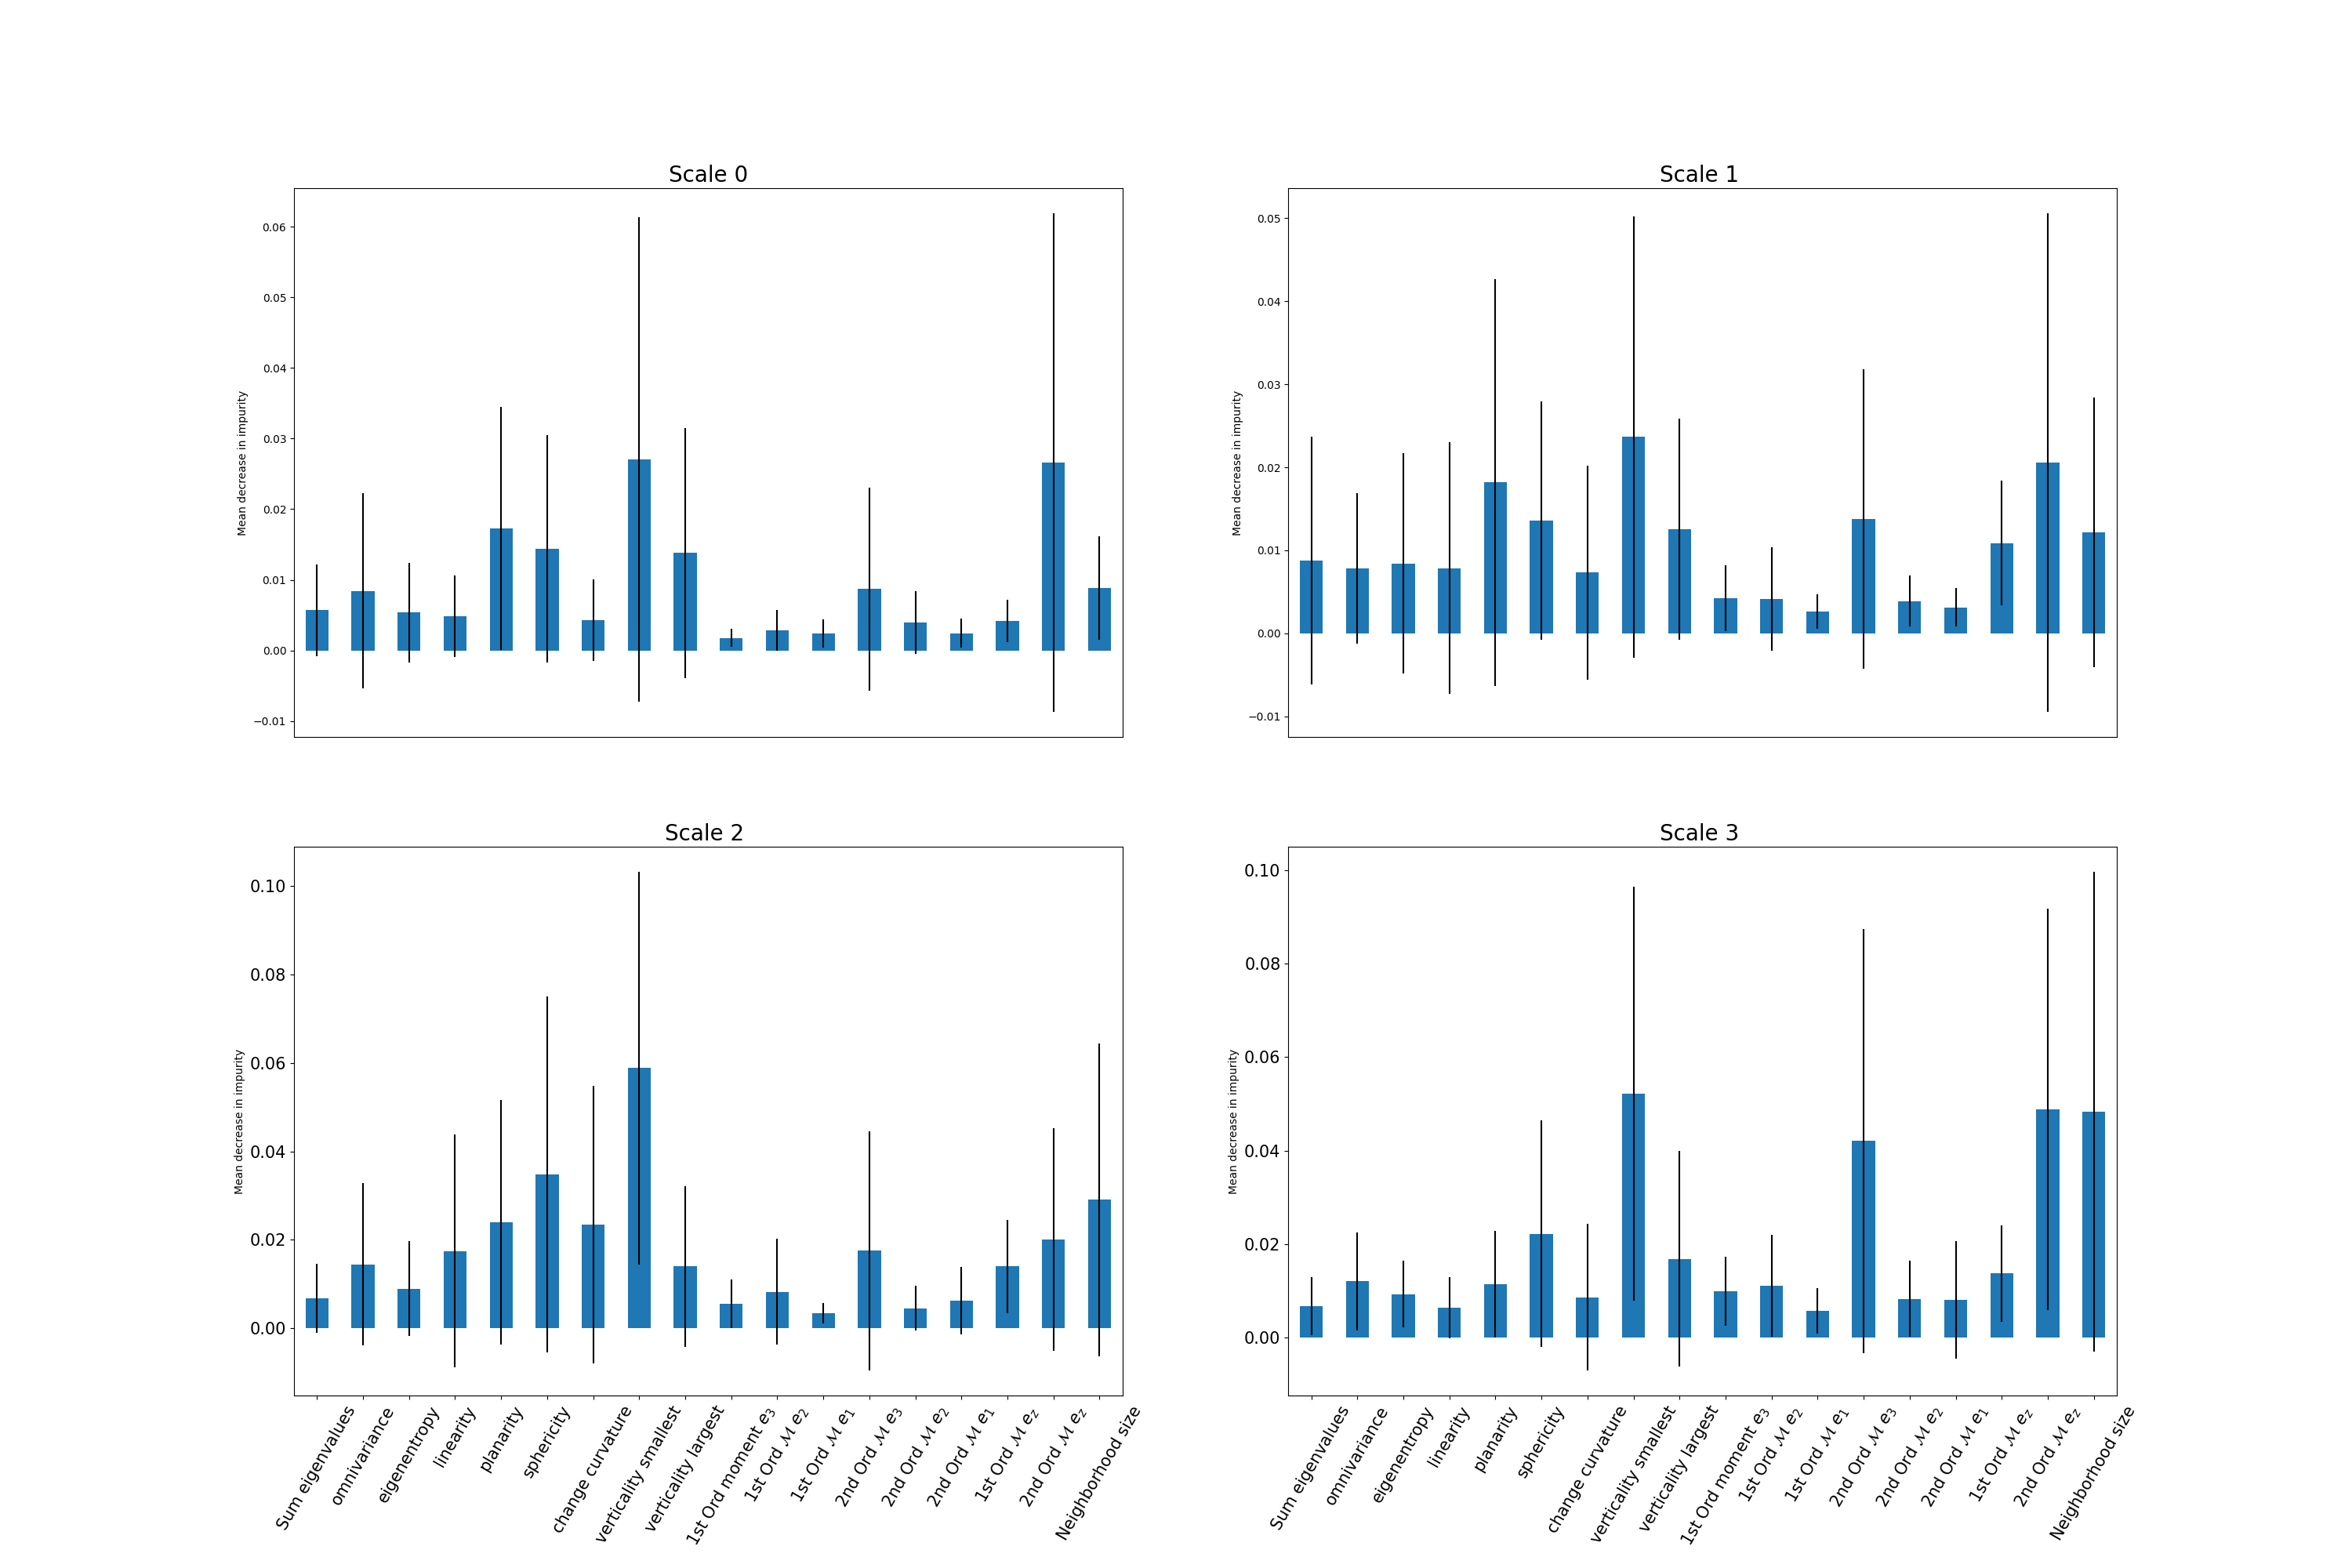
\includegraphics[width=1.3\textwidth]{MDI_feature_importances_DEFAULT.png}
        \caption{MDI feature importances with the 18 features at each scale defined in Table \ref{tab:thomas_feat}. $\mathcal{M}$ refers to the moment. }
        \label{fig:MDI_default}
\end{figure}

\begin{figure}
    \hspace*{-2cm}
        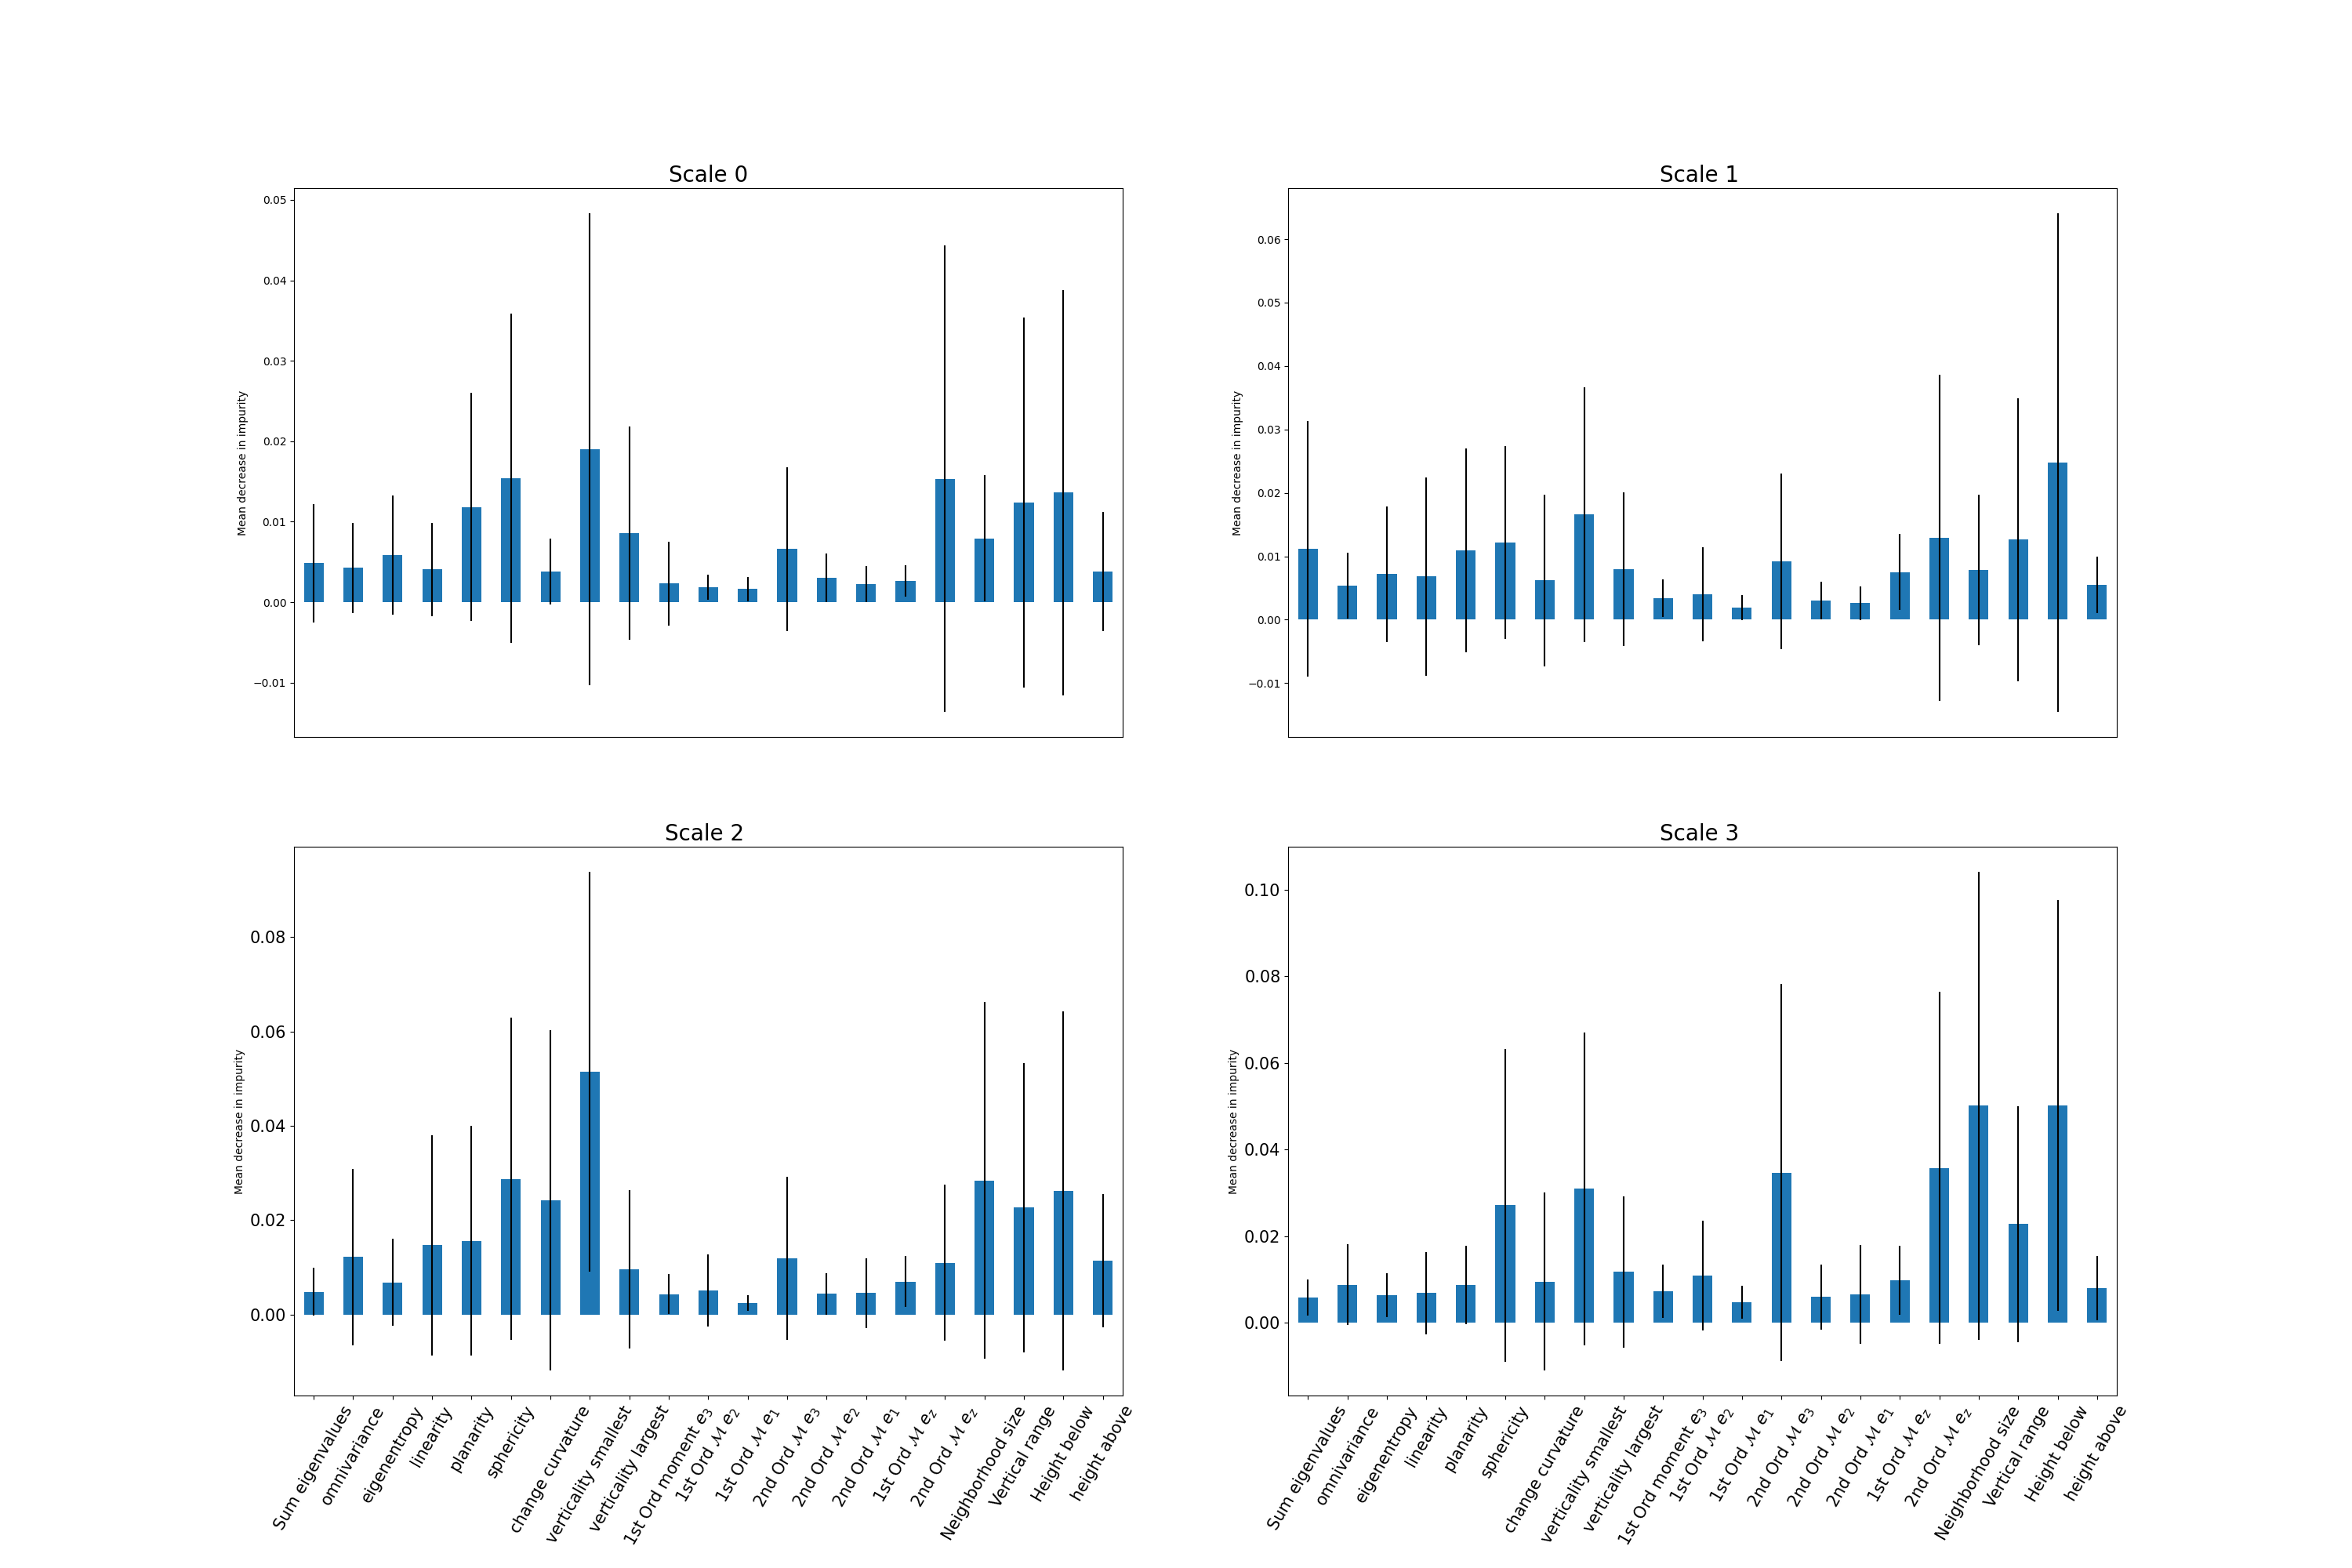
\includegraphics[width=1.3\textwidth]{MDI_feature_importances_W_HEIGHT_FEAT.png}
    \caption{MDI feature importances for the Paris-rue-Cassette dataset with additional height features (21 features in total).}
    \label{fig:MDI_height}
\end{figure}

Feature importances can be computed as the mean and standard deviation of the accumulation of impurity decrease within each tree. Impurity decrease refers to the reduction in the criterion value\footnote{Here, it is the Gini index} when a feature is used to split a node in a decision tree. The importance of a feature is calculated as the (normalized) total reduction of the criterion brought by that feature.

Figures \ref{fig:MDI_default} and \ref{fig:MDI_height} display the Mean Decrease Impurity (MDI) feature importances and their standard deviation, respectively for the 18 features of the proposed method \cite{thomas_semantic_2018} and the 21 features including the height features, for each scale. 

In Figure \ref{fig:MDI_default}, the feature at the original scale are less important that the feature at smallest scales. Moreover, the "Number of points" gets more important as the scale decreases, validating the interest of using this new feature. Figure \ref{fig:MDI_height} highlights that the importances of height features are not negligible, especially at the smallest scale. This underscores the value of including more height information in the feature set. 


Permutation feature importance is a common method used to assess the significance of features in a classifier prediction, regardless of the model being used. The main idea is to assess how much the model's performance changes when modifying the value of the given feature. This is achieved by randomly shuffling the values of the feature and observing the resulting change in prediction accuracy.
Unlike the previous method, this approach is not biased by high-cardinality features, ie variables with a high level of diversity in their values.

Figures \ref{fig:permutation_default} and \ref{fig:permutation_height} display the permutation feature importances and their standard deviation for the same features. 

It is noteworthy that the verticality of the smallest eigenvector $e_3$ exhibits a significant MDI and permutation feature importance at almost every scales. This observation is consistent with findings in \cite{thomas_semantic_2018}, where it was noted that the verticality of the smallest eigenvectors encodes information about the normal vector's orientation of planar objects. This feature's importance stems from its ability to capture the orientation of objects relative to the ground, which can be crucial for distinguishing between different classes, such as 'Motorcycles', 'Pedestrians', and 'Cars'.

\begin{figure}
    \hspace*{-2cm}
    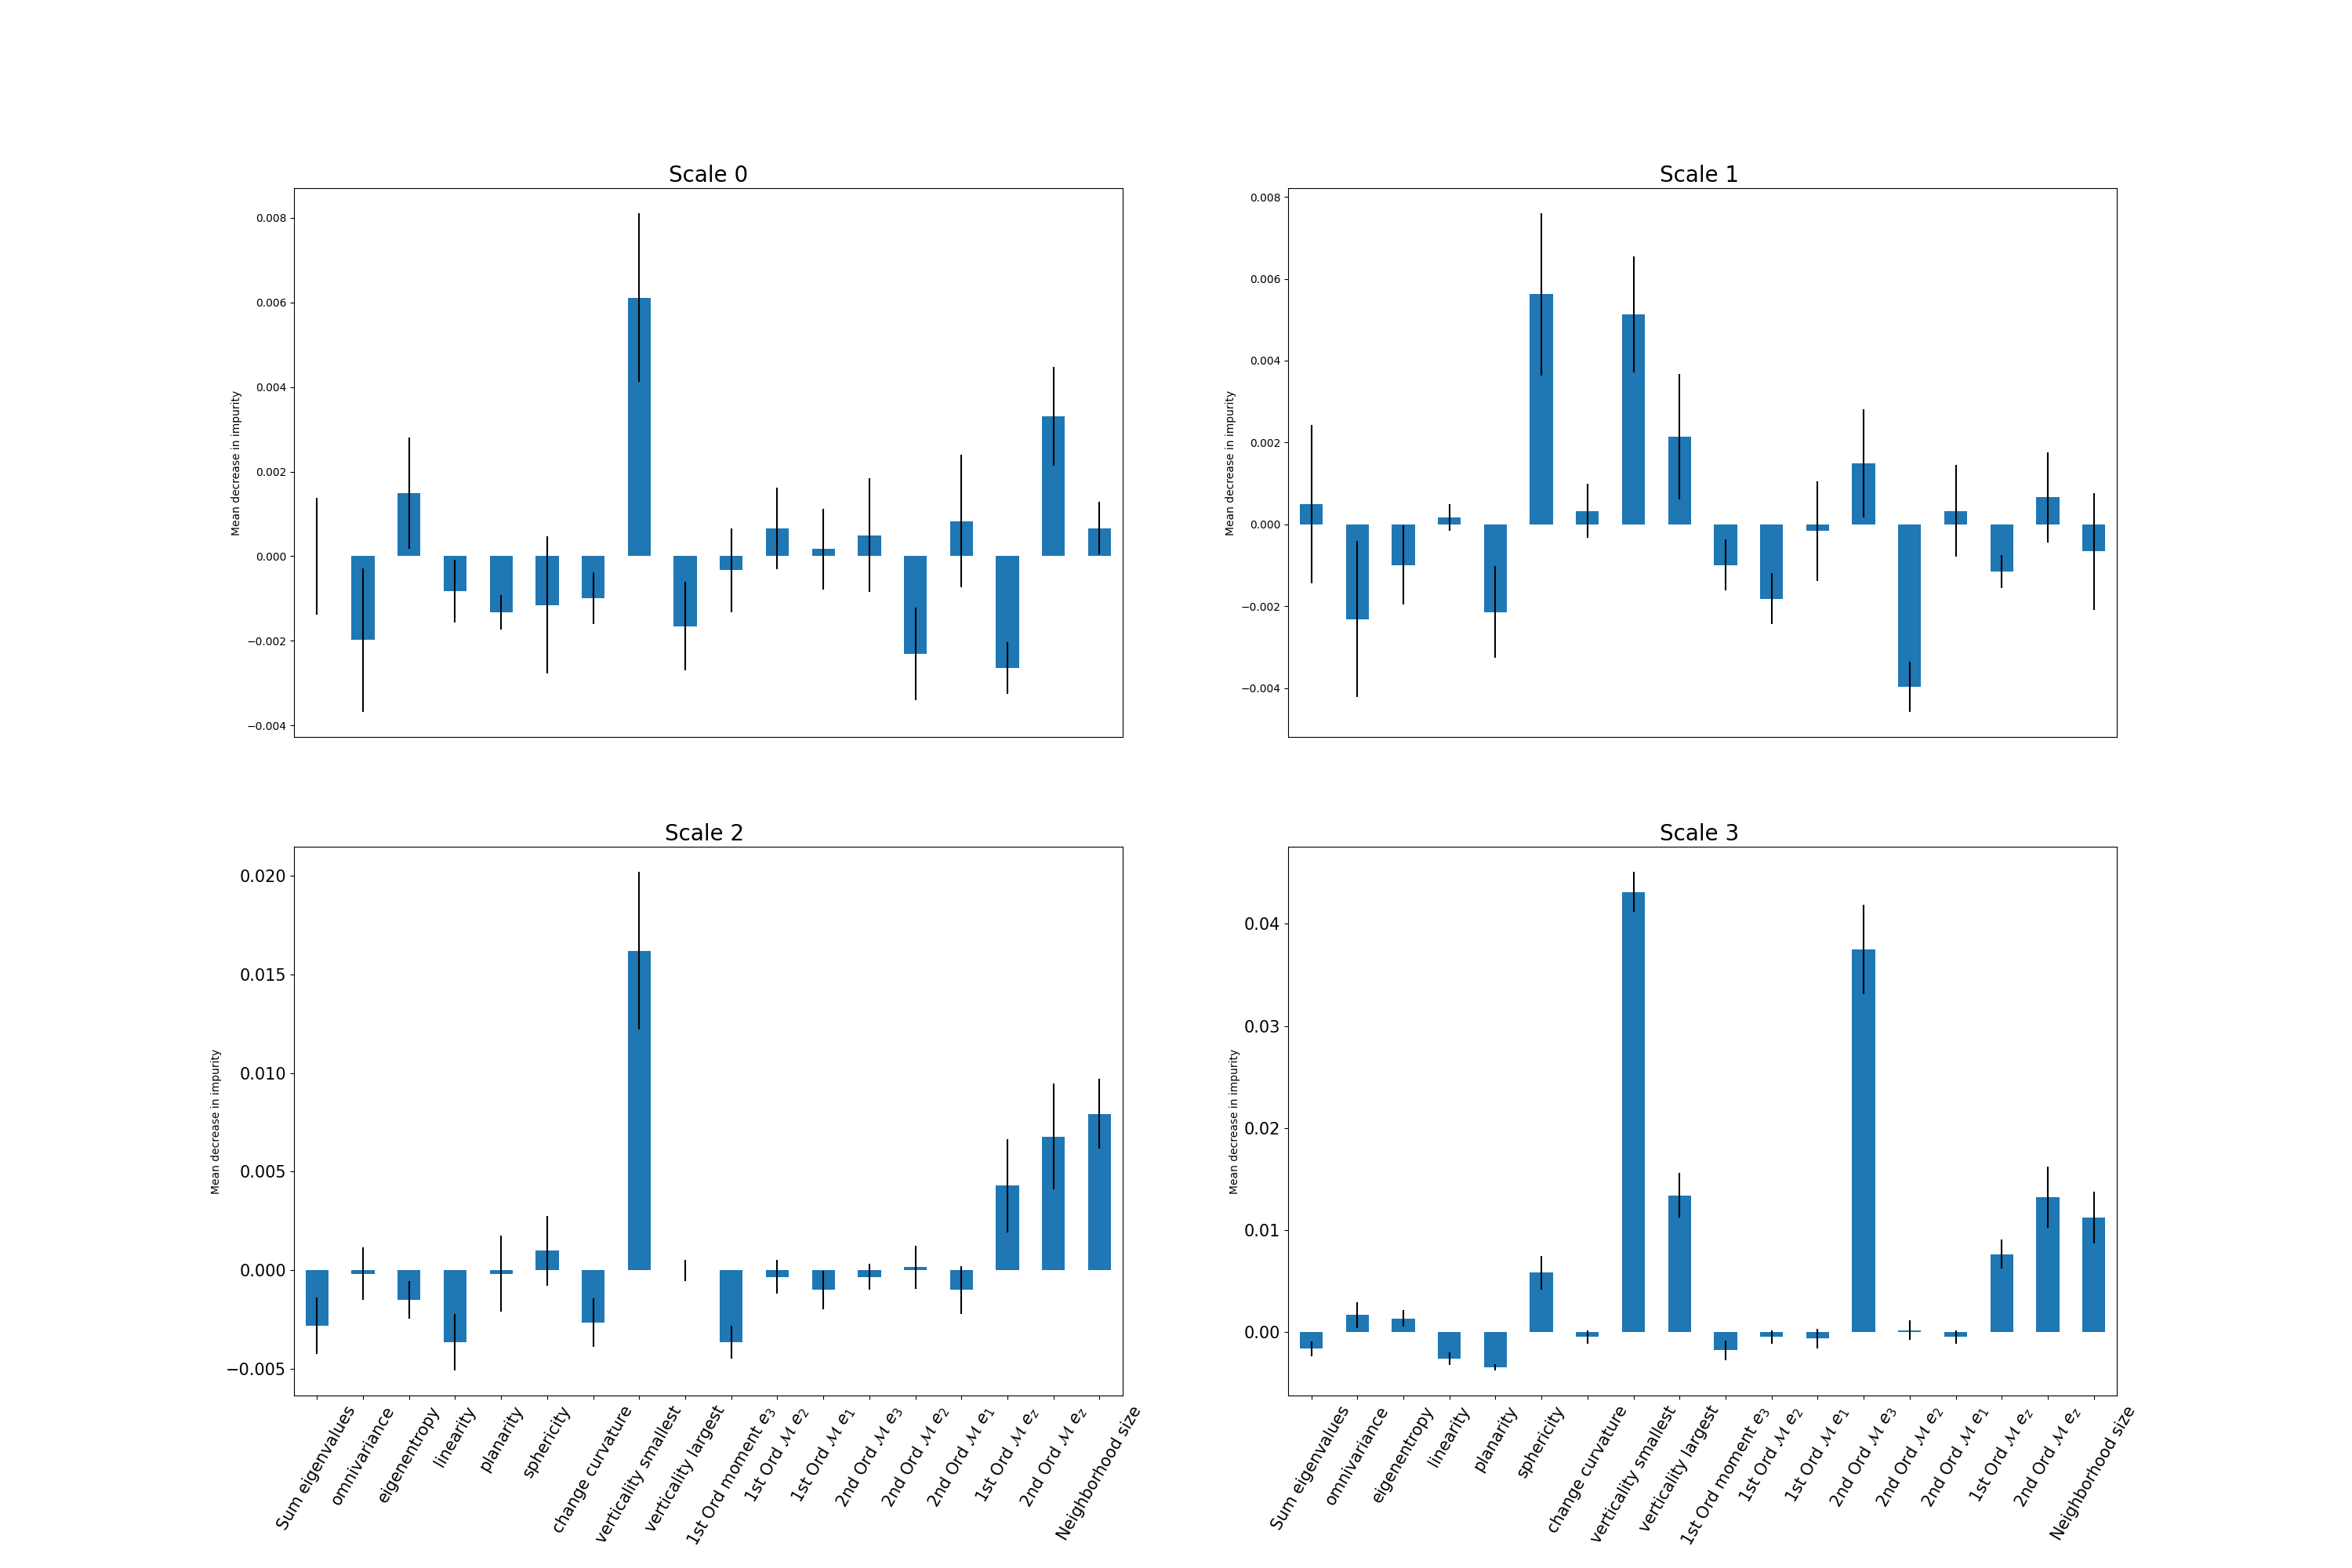
\includegraphics[width=1.3\textwidth]{permutation_feature_importances_DEFAULT.png}
    \caption{Permutation feature importances with the 18 features used in \cite{thomas_semantic_2018} at each scale. $\mathcal{M}$ refers to the moment.}
    \label{fig:permutation_default}
\end{figure}
\begin{figure}
    \hspace*{-2cm}
        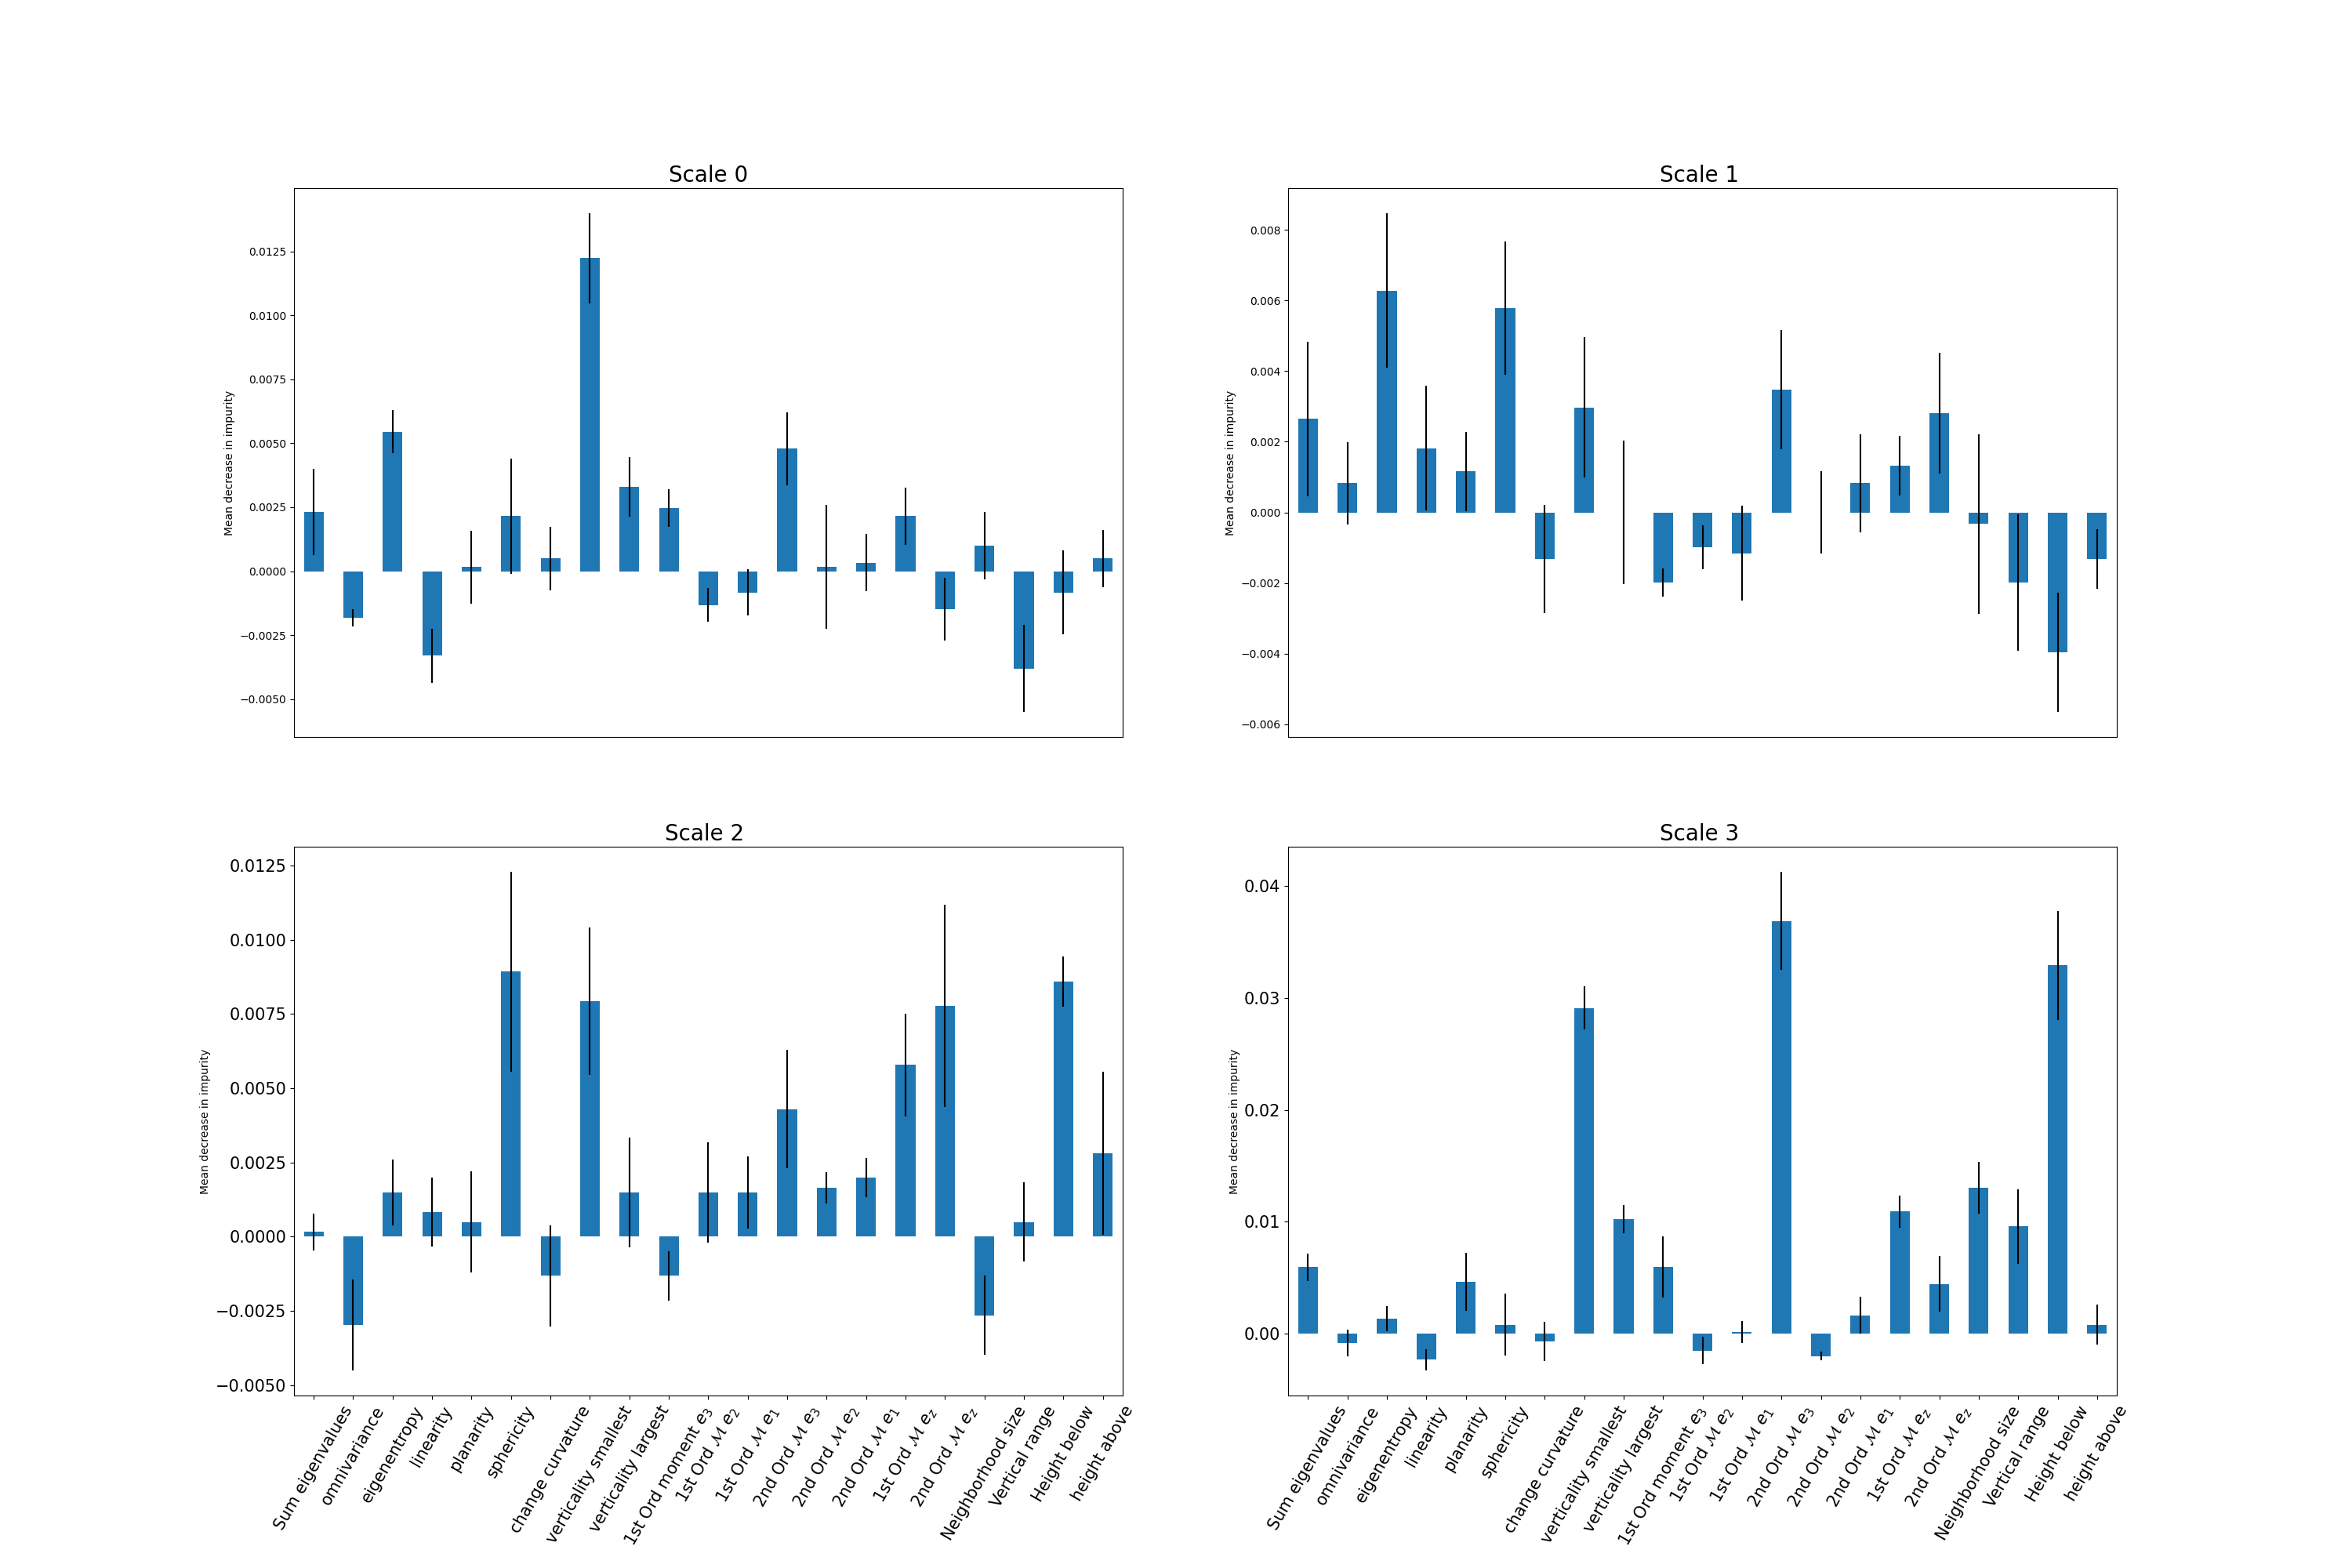
\includegraphics[width=1.3\textwidth]{permutation_feature_importances_W_HEIGHT_FEAT.png}
    \caption{Permutation feature importances for the Paris-rue-Cassette dataset with additional height features (21 features in total for each scale). $\mathcal{M}$ refers to the moment.}
    \label{fig:permutation_height}
\end{figure}




\subsection{NPM3D dataset and generalization on an Unseen point clouds}\label{sec:generalization}

For this experiment, I have randomly selected 100,000 points per class from the MiniLille dataset to train the Random Forest classifier. Here, the number of scales is $S=3$, $r_0=0.8$, $\phi=2$, $\rho=5$ and I used a spherical neighborhood. To assess the generalization ability of the method, I considered points in the MiniParis point cloud with a non-zero labels. Subsequently, I predicted the labels of 34,7651 points from this dataset. The results are presented in Table \ref{tab:results_generalization}. 

The classifier trained on the MiniLille dataset generalizes well to the MiniParis dataset, with a weighted IoU score of 97.89\%. This demonstrates the robustness of the proposed method and its ability to generalize to unseen datasets. 

The computation of features for the test points required 4 hours, while the training of the classifier itself took 49 minutes. These processing times reflect the computational resources necessary for the feature extraction and training phases when dealing with a large number of points.


\begin{table}[H]
    \centering
\begin{tabular}{cc}
    Classes & IoU \\
    \hline\hline
    Ground & 98.41\% \\
    Building & 97.44\% \\
    Poles & 98.40\% \\
    Pedestrians & 98.34\% \\
    Cars & 98.85\% \\
    Vegetation & 96.86\% \\
    \hline 
    Weighted IoU & 97.89\% \\
\end{tabular}
\caption{IoU on the MiniParis dataset using the Random Forest classifier trained on the MiniLille dataset. Here, the number of scales is $S=3$, $r_0=0.8$, $\phi=2$, $\rho=5$.}
\label{tab:results_generalization}
\end{table}

\section{Improvement proposals}\label{sec:classification}

One of the requirements for this project was to propose improvements to the method. I have proposed and implemented the addition of height features to the feature set. The results were discussed in section \ref{sec:compare_w/o_height}.

\textbf{Speed up attempts.} I also tried to speed up the feature computation code. I computed the features on multiple CPU processes using \texttt{multiprocessing} package to speed up loops. Howerver, objects placed on multiprocessing queues are pickled, transferred over the queue, and then unpickled. The pickling and unpickling steps add overhead, and for large objects this overhead can be significant. This is because large objects require more data to be pickled and transferred, and the unpickling step requires reconstructing the entire object. 

Then, I tried Numba which is a just-in-time compiler for Python that works best on code that uses NumPy arrays and functions. Computing the features of 40 points with 4 scales on the subsampled Paris-rue-Cassette point cloud (about 1,288,215 points) took 54 seconds. I computed and saved the features of all points, excluding the points with label 0. 

\textbf{Classification methods.} Random Forest classifier is usually used for semantic classification of 3D point clouds \cite{thomas_semantic_2018,hackel_fast_nodate}. Indeed, it is directly applicable to multi-class problems and has been shown to yield good results in reasonable time on large point clouds \cite{weinmann_semantic_2015,atik_machine_2021}. I use Gini index as splitting criterion.

However, other classification methods could be considered \cite{atik_machine_2021}. 

Boosting is an ensemble machine learning approach. Boosting algorithms combine multiple low accuracy or weak models to create high accuracy or strong model. Among the most popular boosting algorithms are AdaBoost, Gradient Boosting, and XGBoost.

\section{Conclusion}

In 2019, Thomas et al. \cite{thomas_kpconv_2019} propose a deep learning approach for semantic segmentation using convolutions on point clouds.

In conclusion, our investigation into semantic classification using multiscale features has yielded valuable insights into the effectiveness of various feature extraction methods and their impact on classification performance. Through comparative analysis, we have demonstrated the superiority of employing spherical neighborhoods over KNN methods, emphasizing the importance of contextual information in accurately characterizing point cloud data. Additionally, our assessment of additional features, such as height features, has underscored their significance in capturing vertical characteristics, thereby enhancing classification accuracy. Importantly, our findings align with previous research, highlighting the importance of considering spatial orientation in distinguishing between different object classes.

Moving forward, the insights gained from this project can inform the development of more robust and accurate semantic classification algorithms for point cloud data analysis. By incorporating multiscale features and leveraging contextual information effectively, we can enhance the performance of classification models across various real-world applications, from autonomous driving to urban planning and beyond. As technology continues to advance, the integration of sophisticated feature extraction techniques will play a crucial role in unlocking the full potential of point cloud data analysis in diverse domains.

\newpage
\bibliographystyle{plain}
\bibliography{ref}



\end{document}